%Este trabalho está licenciado sob a Licença Atribuição-CompartilhaIgual 4.0 Internacional Creative Commons. Para visualizar uma cópia desta licença, visite http://creativecommons.org/licenses/by-sa/4.0/deed.pt_BR ou mande uma carta para Creative Commons, PO Box 1866, Mountain View, CA 94042, USA.

\chapter{Multiprocessamento (MP)}\label{cap_mp}
\thispagestyle{fancy}

Neste capítulo, vamos estudar aplicações da computação paralela em arquitetura de memória compartilhada. Para tanto, vamos discutir código C/C++ com a API \href{https://www.openmp.org/}{OpenMP}.

\section{Olá, Mundo!}\label{sec_ola_cap_mp}

A computação paralela com MP inicia-se por uma instância de processamento \emph{thread master}. Todas as instâncias de processamento disponíveis (\emph{threads}) leem e escrevem variáveis compartilhadas. A ramificação ({\it fork}) do processo entre os {\it threads} disponíveis é feita por instrução explícita no início de uma região paralela do código. Ao final da região paralela, todos os {\it threads} sincronizam-se ({\it join}) e o processo segue apenas com o {\it thread master}. Veja a Figura \ref{fig:mpwf}.

\begin{figure}[H]
  \centering
  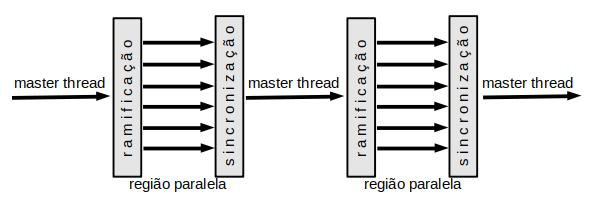
\includegraphics[width=0.7\textwidth]{./cap_mp/dados/fig_mpwf/mpwf}
  \caption{Fluxograma de um processo MP.}
  \label{fig:mpwf}
\end{figure}

Vamos escrever nosso primeiro programa MP. O Código \verb+ola.cc+ inicia uma região paralela e cada instância de processamento escreve ``Olá'' e identifica-se.

\lstinputlisting[title={Código: ola.cc}]{cap_mp/dados/cc_ola/ola.cc}

Na linha 4, o API OpenMP é incluído no código. A região paralela vale dentro do escopo iniciado pela instrução
\begin{verbatim}
# pragma omp parallel
\end{verbatim}
i.e., entre as linhas 12 e 17. Em paralelo, cada {\it thread} registra seu número de identificação na variável \verb+id+, veja a linha 14. Na linha 16, escrevem a saudação, identificando-se.

Para compilar este código, digite no terminal
\begin{verbatim}
$ g++ -fopenmp ola.cc
\end{verbatim}

Ao compilar, um executável \verb+a.out+ será criado. Para executá-lo, basta digitar no terminal:
\begin{verbatim}
$ a.out
\end{verbatim}

Ao executar, devemos ver a saída do terminal como algo parecido com\footnote{O código foi rodado em uma máquina Quadcore com 4 {\it threads}.}
\begin{verbatim}
Processo 0, olá!
Processo 3, olá!
Processo 1, olá!
Processo 2, olá!
\end{verbatim}

A saída irá depender do número de {\it threads} disponíveis na máquina e a ordem dos {\it threads} pode variar a cada execução. Execute o código várias vezes e analise as saídas!

\begin{obs}
  As variáveis declaradas dentro de uma região paralela são privadas de cada {\it threads}. As variáveis declaradas fora de uma região paralela são globais, sendo acessíveis por todos os {\it threads}.
\end{obs}

\subsection*{Exercícios resolvidos}

\begin{exeresol}
  O número de instâncias de processamento pode ser alterado pela variável do sistema \verb+OMP_NUM_THREADS+. Altere o número de {\it threads} para 2 e execute o Código ola.cc.
\end{exeresol}
\begin{resol}
  Para alterar o número de {\it threads}, pode-se digitar no terminal
\begin{verbatim}
$ export OMP_NUM_THREADS=2
\end{verbatim}
  Caso já tenha compilado o código, não é necessário recompilá-lo. Basta executá-lo com
\begin{verbatim}
$ ./a.out
\end{verbatim}
  A saída deve ser algo do tipo
\begin{verbatim}
Olá, processo 0
Olá, processo 1
\end{verbatim}
\end{resol}

\begin{exeresol}
  Escreva um código MP para ser executado com 2 {\it threads}. O {\it master thread} deve ler dois números em ponto flutuante. Então, em paralelo, um dos {\it threads} deve calcular a soma dos dois números e o outro thread deve calcular o produto.
\end{exeresol}
\begin{resol}
\lstinputlisting[title={Código: sp.cc}]{cap_mp/dados/cc_exeresol_sp/sp.cc}  
\end{resol}

\subsection*{Exercícios}

\begin{exer}
  Defina um número de {\it threads} maior do que o disponível em sua máquina. Então, rode o código \verb+ola.cc+ e analise a saída. O que você observa?
\end{exer}

\begin{exer}
  Modifique o código \verb+ola.cc+ de forma que cada {\it thread} escreva na tela ``Processo ID de NP, olá!'', onde ID é a identificação do {\it thread} e NP é o número total de {\it threads} disponíveis. O número total de {\it threads} pode ser obtido com a função OpenMP
\begin{verbatim}
omp_get_num_threads();
\end{verbatim}
\end{exer}

\begin{exer}
  Faça um código MP para ser executado com 2 threads. O {\it master thread} deve ler dois números $a$ e $b$ não nulos em ponto flutuante. Em paralelo, um dos {\it thread} de computar $a-b$ e o outro deve computar $a/b$. Por fim, o {\it master thread} deve escrever $(a-b) + (a/b)$.
\end{exer}

\emconstrucao